% Physics experiment report
% 18/Nov/2016

\documentclass[a4paper,10pt,notitlepage]{article}

\usepackage{CJKutf8}
\usepackage{amsmath}
\usepackage[section]{placeins}
\usepackage{indentfirst}
\usepackage{graphicx}
\usepackage{longtable}

\setlength{\parindent}{2em} 

\begin{CJK*}{UTF8}{gbsn}
\begin{document}

\title{迈克尔逊干涉仪实验报告}
\author{秦光辉\ 9组3号}
\maketitle

\section{实验操作}

\subsection{迈克尔逊干涉仪调节步骤}

\begin{enumerate}
	\item 调整反射镜$M_1$, $M_2$的粗调螺钉及$M_2$的细调螺钉至中间适当位置, 不至于过紧也不至于过松.
	\item 将光阑放到激光器旁边, 调节光阑高度使得光线正好通过小孔. 将光阑放到迈克尔逊干涉仪旁边, 调节激光器仰角使得光线通过小孔. 反复重复上述步骤, 直到激光器和小孔位于同一高度且激光器完全水平.
	\item 自准直法调节$M_1$, $M_2$垂直, 令激光束打在$M_2$的中央部位, 调整$M_1$, $M_2$的粗调螺钉, 使两组反射亮斑的中间亮斑均与光阑的小孔重合。
\end{enumerate}

\subsection{非定域干涉圆条纹和椭圆条纹的调节步骤, 圆条纹的变化规律及解释}

\begin{enumerate}
	\item 在光阑和迈克尔逊干涉仪之间加一个显微镜目镜, 调节目镜位置使得光线尽可能照向$M_2$中心.
	\item 用光屏E接收像, 调节$M_2$的细调螺丝, 使得干涉条纹的圆心大致位于光屏E的中心. 此时两个虚光源的连线和E垂直, 可以观察圆条纹.
	\item 稍稍转动屏, 可接收到椭圆条纹.
	\item 调节粗调手轮, 使得$M_1$在导轨上移动,可观察到圆条纹的吞吐. 当两虚点光源的间距增大时条纹中心亮斑的光程差变大条纹吐, 缩小时条纹中心亮斑的光程差变小, 条纹吞. 还可观察到条纹疏密的变化, 当两虚点光源的间距增大时变密, 缩小时变疏. 
\end{enumerate}

\subsection{非定域直条纹和双曲条纹的调节方法}

\begin{enumerate}
	\item 调节$M_1$的位置, 使得条纹变粗, 最终屏幕E上只留下一到两个条纹.
	\item 用微调螺钉调整$M_2$的俯仰(或偏转), 使两虚点光源连线与屏夹角变小, 夹角变小的过程中椭圆条纹逐渐过渡到双曲条纹. 
	\item 再细调$M_1$的位置, 使得两个虚光源连线和E几乎平行. 此时可以看到直条纹.
\end{enumerate}

\subsection{定域干涉等倾条纹的调节方法, 等倾条纹的变化规律及解释}

\begin{enumerate}
	\item 在非定域干涉下调节$M_1$使得圆条纹较疏. 
	\item 把毛玻璃屏入在扩束透镜与分束镜$G_1$之间, 使光束散射成为扩展光源. 此时干涉条纹出现在无限远处, 用眼睛即可以观察到圆条纹.
	\item 上下左右移动头部, 观察是否有条纹吞吐. 如果有吞吐则细调$M_2$的倾角, 直到吞吐现象消失.
	\item 旋转粗调手轮, 使$M_1$在导轨上移动, 可观察到圆条纹的吞吐. 当反射镜$M_1$由远端移向近端的过程中, 由于两个虚光源逐渐接近, 条纹中心亮斑光程差变小, 出现吞条纹现象, 条纹变粗疏. 当$M_1$和$M_2'$接近重合时两个虚光源几乎重合, 没有干涉现象, 条纹消失. 然后$M_1$继续向近端移动, 条纹中心亮斑光程差变大, 开始吐条纹, 条纹由粗疏变得密集. 
\end{enumerate}

\subsection{定域干涉等厚条纹的调节方法, 等厚条纹的变化规律及解释}

\begin{enumerate}
	\item 在圆条纹粗而疏时, 调节$M_2$的细调螺钉使$M_2$有一个很小的偏转.
	\item 转动粗调手轮, 使弯曲条纹往圆心方向移动, 在视场中将出现直线干涉条纹. 调节细调手轮, 使得直线曲率变小, 直到曲率几乎为0. 如果此时继续转动手轮, 可以看到曲率将会转向相反的方向. 
	\item 由于有一个倾角, 两个虚光源的连线不可能和E垂直. 此时如果我们改变$M_1$的的位置, 两个虚光源的连线的延长线将逐渐和E平行, 当平行的时候我们将看到等厚条纹, 如果不平行, 则可以看到向不同方向弯曲的条纹.
\end{enumerate}

\subsection{白光等厚干涉条纹的调节方法及干涉条纹的现象描述}

\begin{enumerate}
	\item 在等厚干涉条纹变直的附近, 打开白光光源照向毛玻璃. 激光器暂时不关闭, 以便于调节. 调节细调手轮使$M_1$缓慢地移动, 直到视场中出现彩色条纹为止. 
	\item 白光被分解成为了不同颜色的条纹. 中心是白色条纹, 周围是彩色条纹. \textbf{条纹中波长较长的部分相对靠外, 如红光.} 
\end{enumerate}

	当粗调旋钮的指针指向整刻度时, 记录细调旋钮的读数为0.00362mm. 当白光的白色条纹出现在中心的时候读数为46.86905mm, 则我们可以得到
	
\begin{equation*}
	D = (46.86905 - 0.00362) mm = 56.86543mm
\end{equation*}

\subsection{实验图片}

\begin{figure}
\centering
	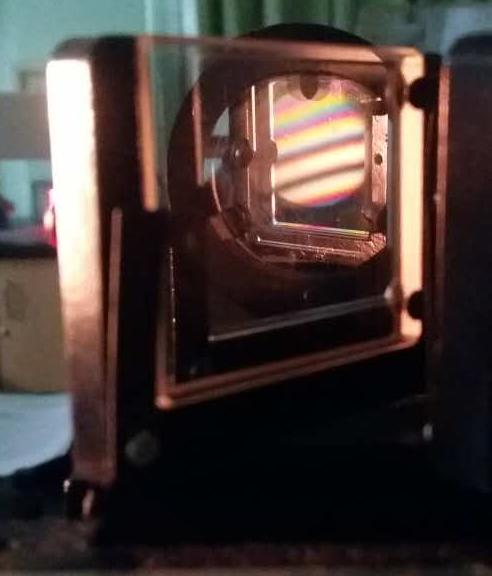
\includegraphics[scale=0.5]{f1.jpg}
	\caption{彩条纹图样}
\end{figure}

\begin{figure}
\centering
	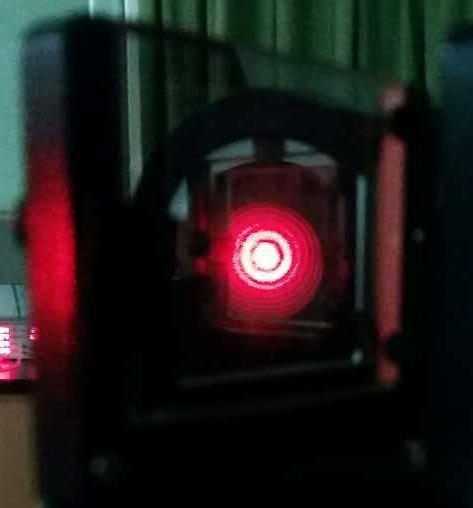
\includegraphics[scale=0.075]{f2.jpg}
	\caption{圆条纹图样}
\end{figure}

\section{数据记录和计算}

\subsection{压电陶瓷的压电常量}

	实验中的仪器参数:
	
\begin{align*}
	L &= 46mm \\
	t &= 1.0mm \\
	\lambda &= 632.8nm
\end{align*}

	测量数据见表一.

\begin{center}

	\begin{longtable}{|c|c|c|c|c|c|c|}
	\caption{压电陶瓷测量数据} \\
	\hline
	n & 1 & 2 & 3 & 4 & 5 & 6 \\
	\hline
	$U_f$/V & 130.6 & 98.2 & 69.7 & 43.8 & 20.3 & 0.0 \\
	\hline
	\hline
	n & 7 & 8 & 9 & 10 & 11 & 12 \\
	\hline
	$U_f$/V & -21.5 & -41.8 & -62.1 & -80.1 & -99.4 & -115.7 \\
	\hline
	\end{longtable}

\end{center}

	作图如图三. \\
	
\begin{figure}
\centering
	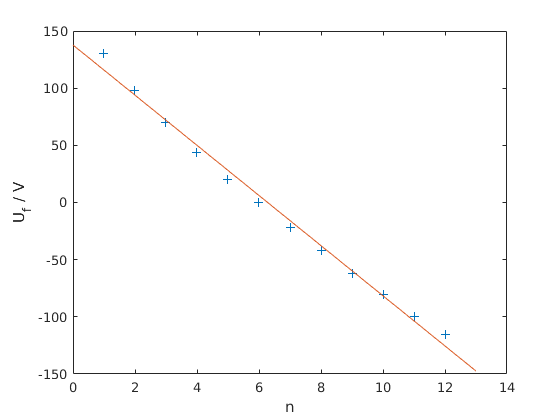
\includegraphics[scale=0.7]{f3.png}
	\caption{压电陶瓷实验数据拟合图线}
\end{figure}

	线性拟合的结果为 \\
	
\begin{align*}
	k &= -21.9357 V \\
	b &= 137.748 V \\
	r &= -0.996035 \\
	\sigma^2 &= \frac{\sum_{i = 1}^{n}(y_i - b - kx_i)^2}{n - 2} = 54.8855 V^2 \\
	\sigma_k &= |k| \times \sqrt{\frac{1/r^2 - 1}{n - 2}} = 0.619528V 
\end{align*}

	由此可以计算压电陶瓷的压电常量
	
\begin{align*}
	d &= \frac{\lambda t}{2|k|L} = 3.136 \times 10^{-10} m/V \\
	\sigma_t &= \frac{e_t}{\sqrt{3}} = 0.0577 mm \\
	\sigma_L &= \frac{e_L}{\sqrt{3}} = 0.577 mm \\
	\sigma_{\lambda} &= \frac{e_{\lambda}}{\sqrt{3}} = 0.0577 nm \\
	\sigma_d &= d \times \sqrt{(\frac{\sigma_k}{k})^2 + (\frac{\sigma_L}{L})^2 + (\frac{\sigma_t}{t})^2 + (\frac{\sigma_{\lambda}}{\lambda})^2} 
	= 0.3 \times 10^{-10} m/V \\
	d \pm \sigma_d &= 3.1 \pm 0.3 \times 10^{-10} m/V
\end{align*}

	由此可见压电陶瓷压电常数为$3.1 \times 10^{-10}$m/V, 误差约为$0.3 \times 10^{-10}$m/V.
	
\subsection{空气折射率的测量}

	实验中的仪器参数:
	
\begin{align*}
	D &= 4.00mm \\
	\lambda &= 632.8nm \\
	p_0 &= 1004 hPa
\end{align*}

	实验中每10个条纹吞吐计数一次, 测量数据见表二.

\begin{center}

	\begin{longtable}{|c|c|c|c|c|c|c|}
	\caption{空气折射率测量数据} \\
	\hline
	$p_i$/hPa & 1386 & 1486 & 1391 & 1354 & 1319 \\
	\hline
	$p_f$/hPa & 1091 & 1163 & 1095 & 1061 & 1023 \\
	\hline
	$\Delta$p/hPa & 295 & 300 & 296 & 293 & 296 \\
	\hline
	\end{longtable}

\end{center}

	可以计算出$\Delta$p均值和不确定度分别为
	
\begin{align*}
	\bar{\Delta p} &= 296 hPa \\
	\sigma_{\bar{\Delta p}} &= 1.0198 hPa \\
\end{align*}

	可以计算出空气的折射率为
	
\begin{align*}
	n &= 1 + \frac{N\lambda p_0}{2D\Delta p} = 1.0002683 \\
	\sigma_D &= \frac{e_D}{\sqrt{3}} = 0.00577 cm \\
	\sigma_{p_0} &= 0.577hPa \\
	\sigma_n &= (n - 1) \times \sqrt{(\frac{\sigma_D}{D})^2 + (\frac{\sigma_{p_0}}{p_0})^2 + (\frac{\sigma_{\Delta p}}{\Delta p})^2 + (\frac{\sigma_{\lambda}}{\lambda})^2} = 1.014 \times 10^{-6} \\
	n &= 1.000268 \pm 0.000002
\end{align*}

	可见空气折射率为$1.000268 \pm 0.000002$.
	
\subsection{激光器波长测量}

	我用干涉仪做了测量氦氖激光器波长的实验. 每50次条纹吞吐测量一次数据, 实验数据见表三.
	
\begin{center}

	\begin{longtable}{|c|c|c|c|c|c|c|}
	\caption{激光器波长测量数据} \\
	\hline
	n & 1 & 2 & 3 & 4 & 5 & 6 \\
	\hline
	x/mm & 35.15868 & 35.14652 & 35.12003 & 35.10748 & 35.09493 & 35.08206 \\
	\hline
	\hline
	n & 7 & 8 & 9 & 10 & 11 & 12 \\
	\hline
	x/mm & 35.06629 & 35.05049 & 35.04456 & 35.01870 & 35.00222 & 34.98600 \\
	\hline
	\end{longtable}

\end{center}

	作图见图四. \\
	
\begin{figure}
\centering
	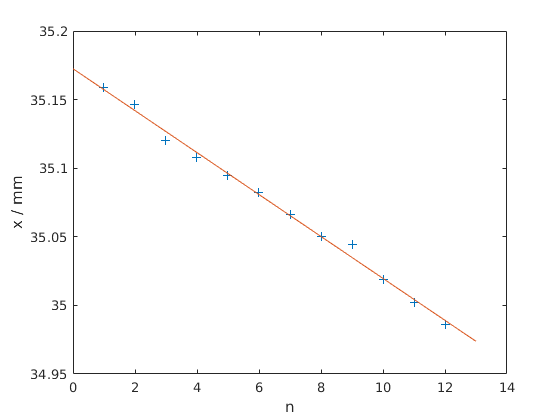
\includegraphics[scale=0.8]{f4.png}
	\caption{测量激光器波长拟合直线}
\end{figure}

	线性拟合的结果为 \\
	
\begin{align*}
	k &= -0.016284 mm \\
	b &= 35.1725 mm \\
	r &= -0.99712 \\
	\sigma^2 &= \frac{\sum_{i = 1}^{n}(y_i - b - kx_i)^2}{n - 2} = 1.93 \times 10^{-5} mm^2 \\
	\sigma_k &= |k| \times \sqrt{\frac{1/r^2 - 1}{n - 2}} = 0.00036763V 
\end{align*}

	由此可以计算氦氖激光器的波长
	
\begin{align*}
	\lambda &= \frac{|k|}{25} = 6.21 \times 10^{-7} m \\
	\sigma_{\lambda} &= \lambda \times \frac{\sigma_k}{|k|} = 0.1599 \times 10^{-7} m \\
	\lambda \pm \sigma_{\lambda} &= 6.2 \pm 0.2 \times 10^{-7} m
\end{align*}

	由此可见氦氖激光器的波长约为620nm, 误差为20nm. 跟实验室数据632.8 nm相比, 我的实验结果覆盖了真值.

\section{实验误差分析}

\subsection{压电陶瓷压电常数测量误差}

\begin{enumerate}
	\item 本实验中主要误差来源为壁厚t, 其对实验误差贡献最大.
	\item 条纹吞吐的误差也很大. 由于实验非常精密, 周围环境嘈杂, 条纹一直在振动, 难以精准测量.
	\item 条纹吞吐的识别没有客观标准, 仅凭主观确定.
\end{enumerate}

\subsection{空气折射率测量误差}

\begin{enumerate}
	\item 这个实验条纹测量数目较多, 是10条. 这样误差就特别小, 条纹吞吐对实验结果误差贡献不大.
	\item 实验中不太好控制气体的进出, 每次的进出量都很大, 不便控制.
\end{enumerate}

\subsection{氦氖激光器波长测量}

\begin{enumerate}
	\item 这个实验的误差非常大, 其线性拟合结果也很不好. 主要出在条纹的吞吐上, 每次测量的时候总是会出现转动手轮但是条纹不吞吐的情况, 我无法理解这种现象出现的原因. 我没有反向旋转, 所以不可能是回程差. 这对计数造成了致命的影响.
	\item 环境的嘈杂让我不能安心计数, 事实上有几个数据我并不确定恰好数了50个条纹.
	\item 万幸的是最后实验数据覆盖了真值, 虽然误差非常大.
\end{enumerate}

\section{思考和感悟}

	这个实验是一个非常有名的实验, 用非常简单的实验仪器可以完成很复杂的工作. 从这个实验中我也认识到光学实验是一类非常考验操作的实验. 光学实验中有很多精密的仪器, 其精密程度甚至达到说话都会使条纹振动. 虽然实验非常困难, 但是按照正确的方法, 我很快就做完了. 我相信只要认真, 不跳步骤, 再精密复杂的实验都可以完成!
	
\end{CJK*}
\end{document}
